\documentclass[color=usenames,dvipsnames]{beamer}

\mode<presentation> {
	
	\usetheme{Madrid}
	
	\usepackage{tikz}
	\usetikzlibrary{shapes.geometric, arrows}
	
	\definecolor{ERC1}{HTML}{C72321}
	\definecolor{ERC2}{HTML}{861719}
	\definecolor{ERC3}{HTML}{FBD7A9}
	\definecolor{ERC4}{HTML}{BA9F7C}
	\definecolor{ERC5}{HTML}{7A6952}
	\definecolor{ERC6}{HTML}{6E9B9E}
	\definecolor{ERC7}{HTML}{0D8085}
	\definecolor{ERC8}{HTML}{19484C}
	\definecolor{ERC9}{HTML}{F0C320}
	\definecolor{ERC10}{HTML}{AF8F19}
	
	
	\tikzstyle{startstop} = [rectangle, rounded corners, minimum width=3cm, minimum height=1cm,text centered, draw=black, fill=ERC8]
	\tikzstyle{io} = [trapezium, text centered, draw=white, fill=white]
	\tikzstyle{process} = [rectangle, minimum width=3cm, minimum height=1cm, text centered, draw=black, fill=ERC9]
	\tikzstyle{decision} = [diamond, minimum width=3cm, minimum height=1cm, text centered, draw=black, fill=ERC10]
	\tikzstyle{arrow} = [thick,->,>=stealth]
	
	
	\setbeamercolor{palette primary}{bg=ERC1,fg=white}
	\setbeamercolor{palette secondary}{bg=ERC2,fg=white}
	\setbeamercolor{palette tertiary}{bg=ERC3,fg=white}
	\setbeamercolor{palette quaternary}{bg=ERC4,fg=white}
	\setbeamercolor{structure}{fg=ERC5} % itemize, enumerate, etc
	\setbeamercolor{section in toc}{fg=ERC6} % TOC sections
	
	%gets rid of bottom navigation bars
	\setbeamertemplate{footline}[frame number]{}
	
	%gets rid of bottom navigation symbols
	\setbeamertemplate{navigation symbols}{}
	
	%gets rid of footer
	%will override 'frame number' instruction above
	%comment out to revert to previous/default definitions
	\setbeamertemplate{footline}{}
	
	% Override palette coloring with secondary
	%\setbeamercolor{subsection in head/foot}{bg=UBCgrey,fg=white}
	
	
	%\usecolortheme{lily}
	\useoutertheme{infolines}
	
}


\usepackage{booktabs} 
\usepackage{tikz}


% Thin fonts
\usepackage{cmbright}
\usepackage[T1]{fontenc}

\definecolor{dark_grey}{gray}{0.5}
%\setbeamercolor{normal text}{fg=dark_grey,bg=white}
\setbeamertemplate{navigation symbols}{}

%\setbeamercolor*{palette primary}{fg=gray!100,bg=gray!10}
%\setbeamercolor*{palette quaternary}{fg=gray!100,bg=gray!10}
%\setbeamercolor*{palette secondary}{fg=gray!100,bg=gray!20}
%\setbeamercolor*{palette tertiary}{fg=gray!100,bg=gray!10}
%\setbeamercolor*{navigation symbols}{fg=white,bg=white}
\usefonttheme{default}


\setbeamertemplate{blocks}[rounded][shadow=false]
%\setbeamercolor{block title}{bg=gray!10}
%\setbeamercolor{block body}{fg=gray,bg=gray!10}
%\setbeamercolor{frametitle}{fg=}

\setbeamertemplate{frametitle}[default][center]

\setbeamertemplate{itemize items}[default]
\setbeamertemplate{enumerate items}[default]

\newcommand{\F}{\mathbb{F}}

\setbeamertemplate{title page}[default][colsep=-4bp,rounded=true]

\title[Workshop - Machine Learning]{ Don't believe the hype? A hands-on introduction to machine-learning in Python}
\subtitle{Open Workshops on Computer Based Systems Modelling}

\author{Johannes Schmidt, Johann Baumgartner}
\institute{Institute for Sustainable Economic Development, BOKU, Vienna}
\date{7.05.2019}
\begin{document}
	
	\begin{frame}{Supervised learning - Exercise Solution} 
	\begin{table}[ht]
		\centering
		\begin{tabular}{c|c}
			Positives&Negatives\\
			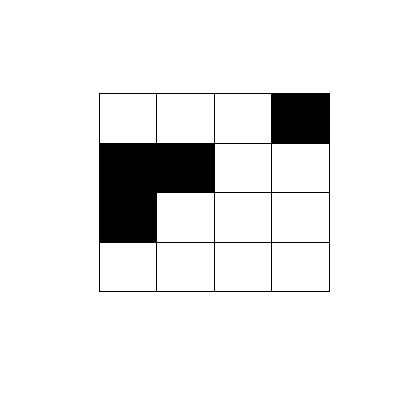
\includegraphics[width=0.1\linewidth]{../figures/2d_pattern_supervised_learning_1.png}
			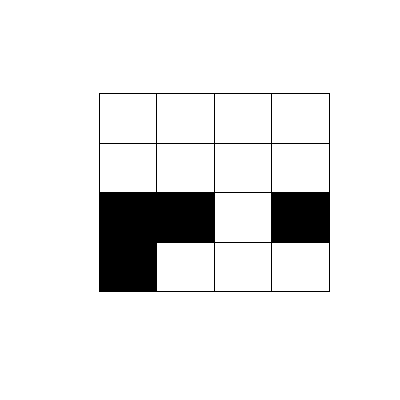
\includegraphics[width=0.1\linewidth]{../figures/2d_pattern_supervised_learning_2.png}
			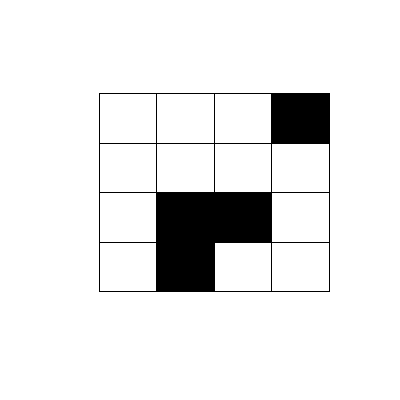
\includegraphics[width=0.1\linewidth]{../figures/2d_pattern_supervised_learning_6.png}
			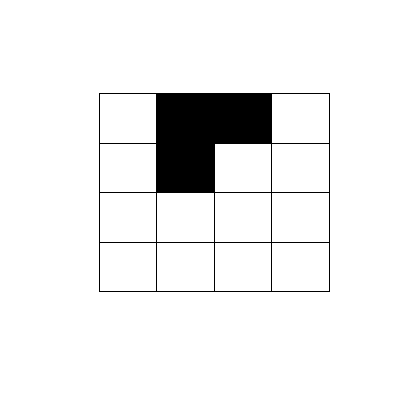
\includegraphics[width=0.1\linewidth]{../figures/2d_pattern_supervised_learning_4.png}&
			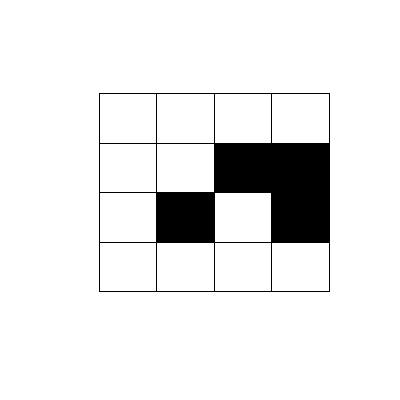
\includegraphics[width=0.1\linewidth]{../figures/2d_random_supervised_learning_1.png}
			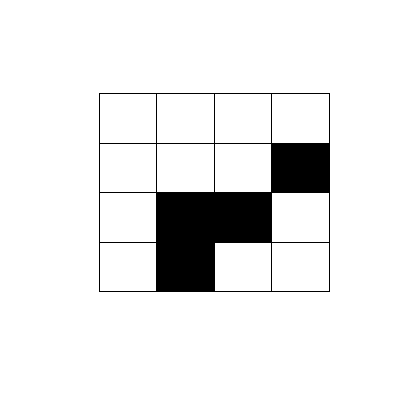
\includegraphics[width=0.1\linewidth]{../figures/2d_random_supervised_learning_2.png}
			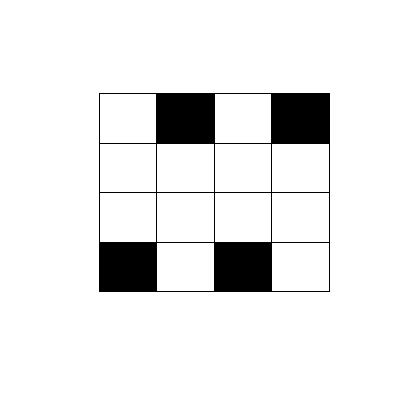
\includegraphics[width=0.1\linewidth]{../figures/2d_random_supervised_learning_3.png}
			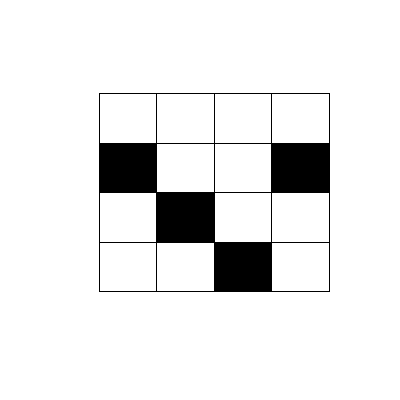
\includegraphics[width=0.1\linewidth]{../figures/2d_random_supervised_learning_4.png}
			\\
		\end{tabular}
	\end{table}
	
	
	
	\begin{center}
		Positive or Negative?\\
		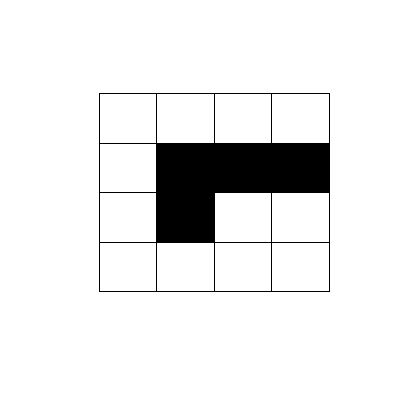
\includegraphics[width=0.1\linewidth]{../figures/2d_pattern_supervised_learning_5.png}
	\end{center}
	
\end{frame}





\end{document}
